\documentclass{article}

\usepackage{graphicx}
\usepackage{tikz}
\usepackage{tikzsymbols}
\usetikzlibrary{calc,patterns,shapes.geometric}
\pagestyle{empty}
\usepackage[margin=0pt]{geometry}
\geometry{papersize={14in,12in}}

\def\centerarc[#1](#2)(#3:#4:#5){\draw[#1] ($(#2)+({#5*cos(#3)},{#5*sin(#3)})$) arc (#3:#4:#5);}

\begin{document}
	\begin{figure}
		\centering
		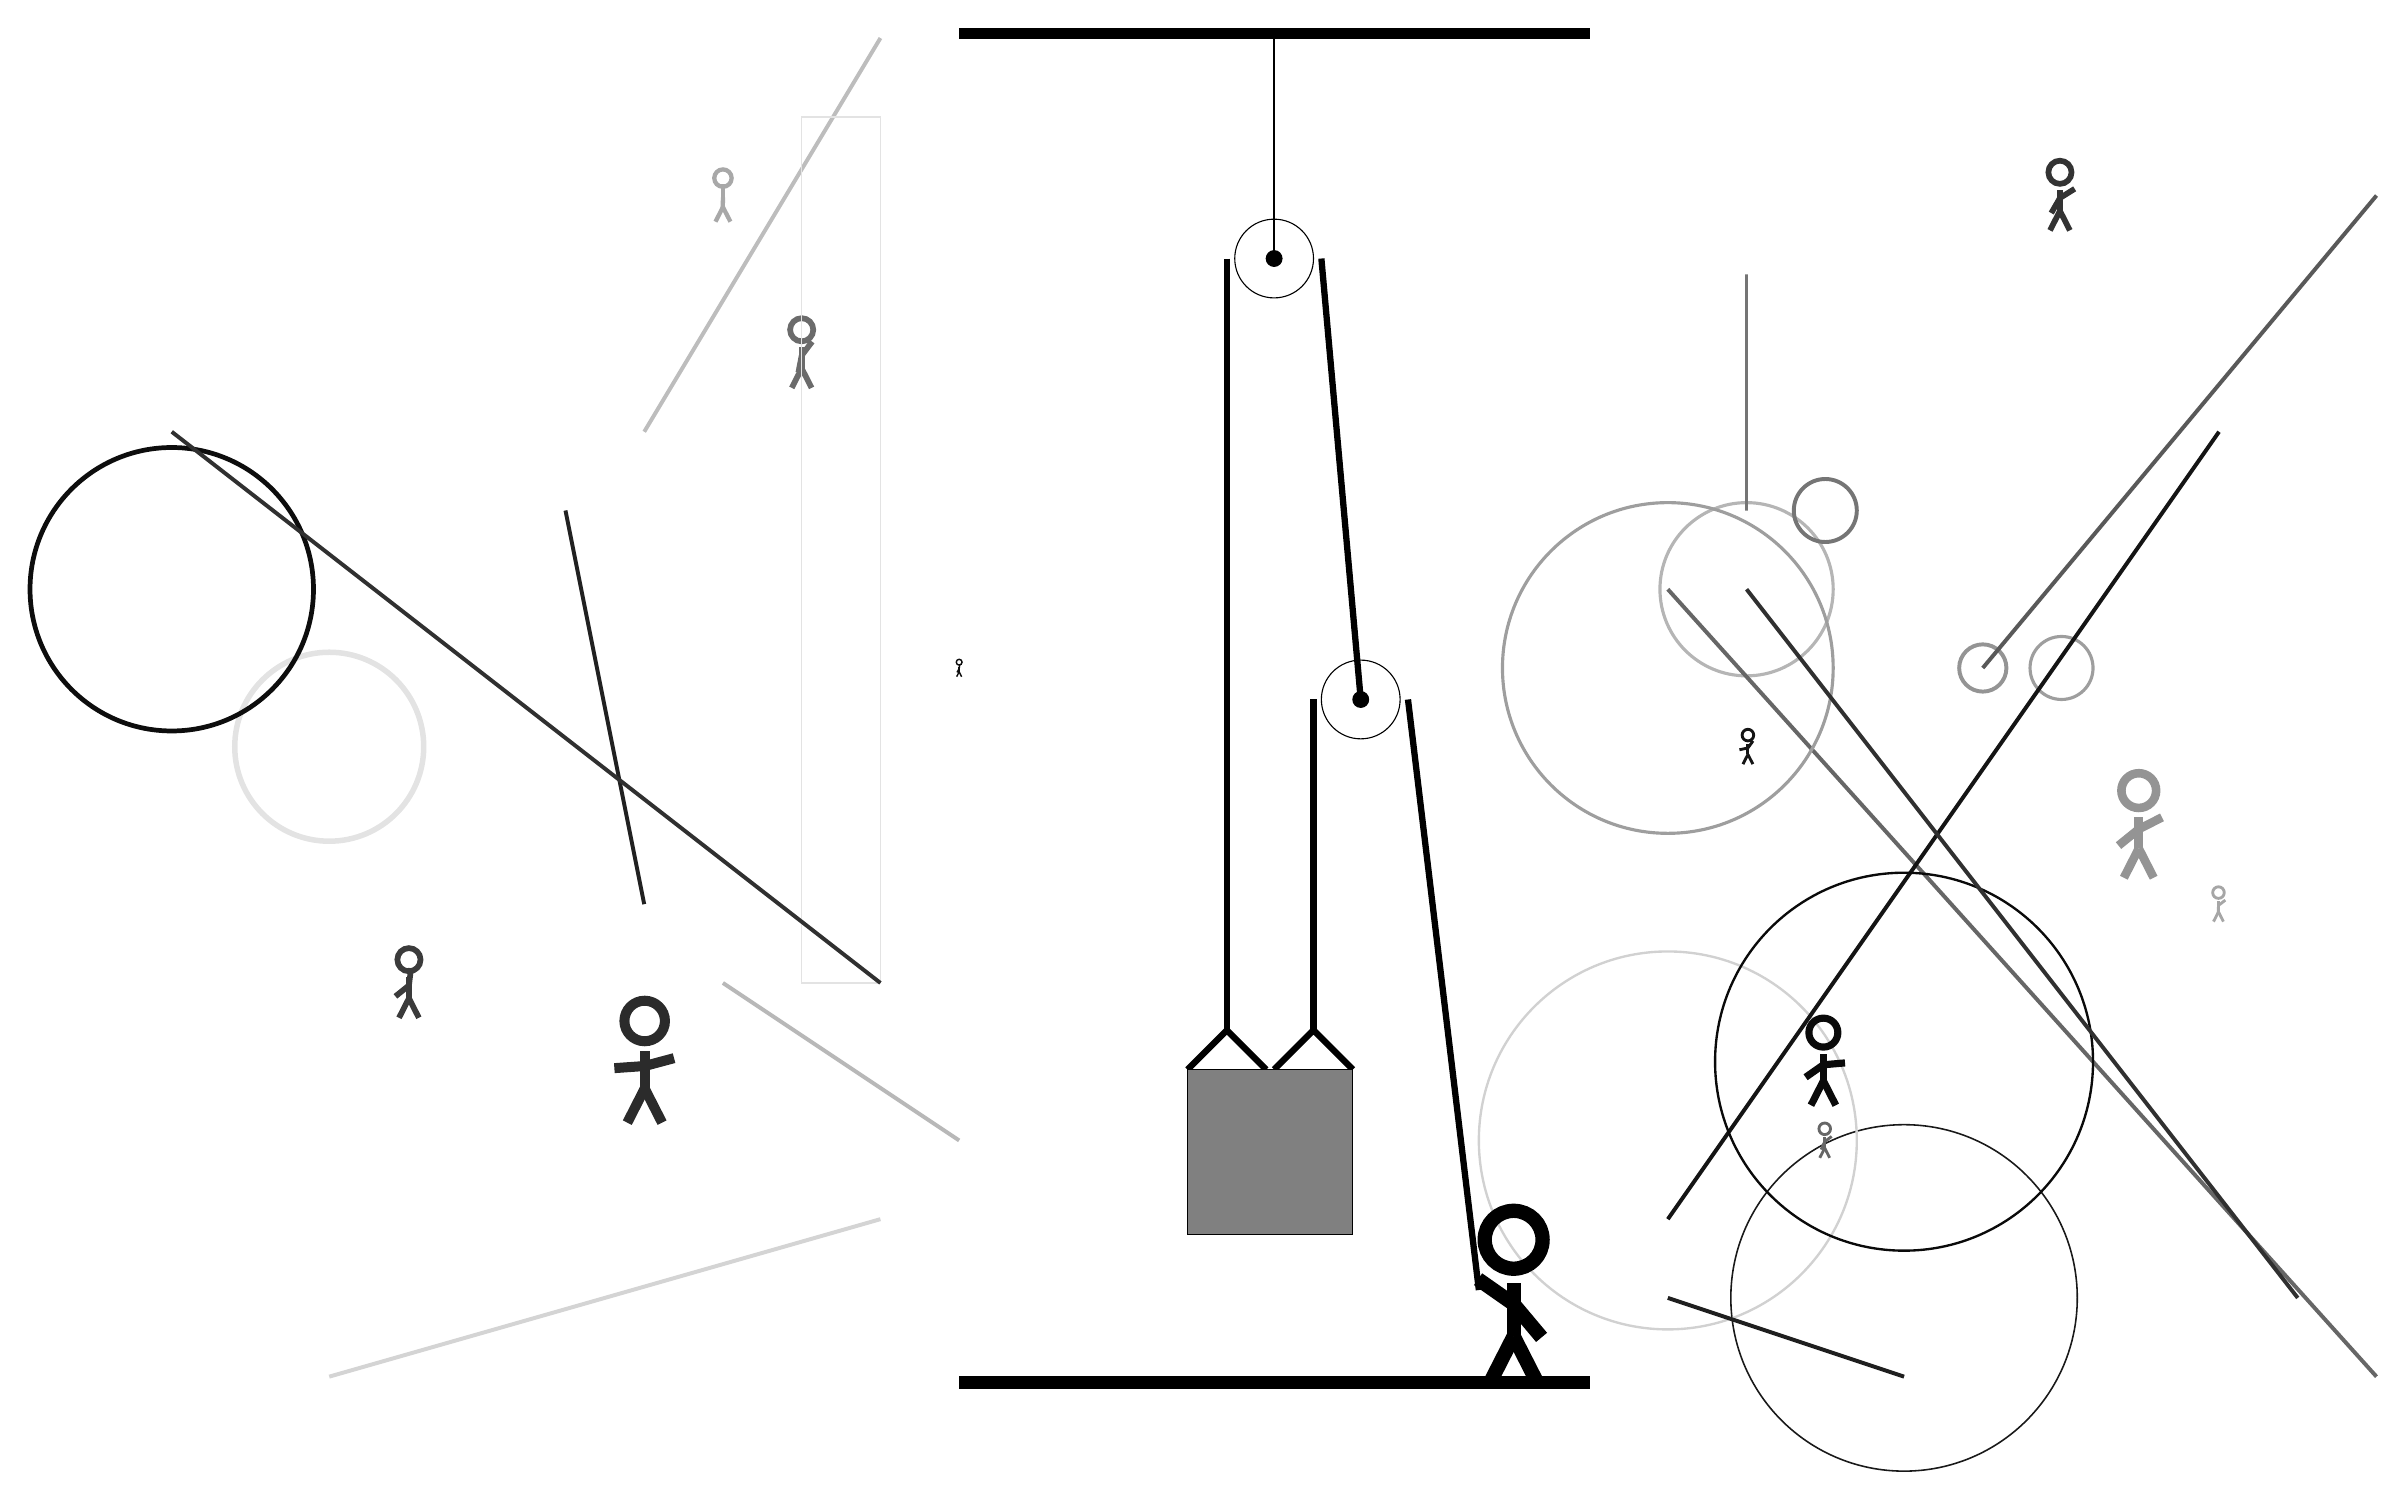
\begin{tikzpicture}
			%%%%% START %%%%%
			
			\draw[fill=black] (-2, 14) rectangle (6, 14.125);
			
			\draw (2, 11.2) circle (0.5);
			\draw[fill=black] (2, 11.2) circle (0.1);
			\draw[thick] (2, 11.2) -- (2, 14);
			
			\draw (3.1, 5.6) circle (0.5);
			\draw[fill=black] (3.1, 5.6) circle (0.1);
			
			\draw [line width=0.2mm, color=black!90](10, -2) circle (2.2);
			
			\draw [line width=0.4mm, color=black!29](8, 7) circle (1.1);
			\draw[line width=0.5mm, color=black!60](7, 7) -- (16, -3);
			\draw[line width=0.3mm, color=black!54] (8, 11) rectangle (8, 8);
			\draw [line width=0.5mm, color=black!42](11, 6) circle (0.3);
			\draw[line width=0.5mm, color=black!87](-7, 8) -- (-6, 3);
			
			\draw [line width=0.3mm, color=black!18](7, 0) circle (2.4);
			\draw [line width=0.5mm, color=black!54](9, 8) circle (0.4);
			\node[line width=0.7mm, color=black!77] at (-9, 2) {\Strichmaxerl[4][39][83]};
			
			\node[line width=0.5mm, color=black!35] at (14, 3) {\Strichmaxerl[2][88][38]};
			\node[line width=0.5mm, color=black!58] at (-4, 10) {\Strichmaxerl[4][79][53]};
			\draw [line width=0.4mm, color=black!38](7, 6) circle (2.1);
			\draw[line width=0.5mm, color=black!17](-3, -1) -- (-10, -3);
			\node[line width=0.5mm, color=black!92] at (8, 5) {\Strichmaxerl[2][12][54]};
			\draw [line width=0.7mm, color=black!11](-10, 5) circle (1.2);
			\draw [line width=0.4mm, color=black!38](12, 6) circle (0.4);
			
			\draw[line width=0.5mm, color=black!92](7, -1) -- (14, 9);
			\node[line width=0.4mm, color=black!96] at (9, 1) {\Strichmaxerl[5][35][5]};
			\draw[line width=0.5mm, color=black!65](11, 6) -- (16, 12);
			
			\draw[line width=0.5mm, color=black!28](-2, 0) -- (-5, 2);
			\draw[line width=0.5mm, color=black!26](-6, 9) -- (-3, 14);
			
			\draw [line width=0.3mm, color=black!96](10, 1) circle (2.4);
			\draw [line width=0.6mm, color=black!95](-12, 7) circle (1.8);
			\node[line width=0.4mm, color=black!95] at (-2, 6) {\Strichmaxerl[1][60][82]};
			\node[line width=0.2mm, color=black!60] at (9, 0) {\Strichmaxerl[2][66][37]};
			
			\draw[line width=0.2mm, color=black!11] (-3, 2) rectangle (-4, 13);
			\draw[line width=0.5mm, color=black!88](10, -3) -- (7, -2);
			\node[line width=0.6mm, color=black!80] at (12, 12) {\Strichmaxerl[4][60][32]};
			\node[line width=0.3mm, color=black!83] at (-6, 1) {\Strichmaxerl[7][4][15]};
			\draw[line width=0.5mm, color=black!81](-3, 2) -- (-12, 9);
			\draw[line width=0.5mm, color=black!81](8, 7) -- (15, -2);
			
			\node[line width=0.3mm, color=black!34] at (-5, 12) {\Strichmaxerl[3][89][90]};
			\node[line width=0.6mm, color=black!42] at (13, 4) {\Strichmaxerl[6][39][27]};
			
			\draw[line width = 0.8mm]  (0.9, 0.9) -- (1.4, 1.4) -- (1.9, 0.9);
			\draw[line width = 0.8mm]  (2.0, 0.9) -- (2.5, 1.4) -- (3.0, 0.9);
			\draw[fill=black!50] (0.9, 0.9) rectangle (3.0, -1.2);
			
			\draw[line width = 0.8mm] (1.4, 11.2) -- (1.4, 1.4);
			\centerarc[line width = 0.8mm](2, 11.2)(0:180:0.6);
			\draw[line width = 0.8mm] (2.6, 11.2) -- (3.1, 5.6);
			\draw[line width = 0.8mm] (2.5, 5.6) -- (2.5, 1.4);
			\centerarc[line width = 0.8mm](3.1, 5.6)(0:180:0.6);
			\draw[line width = 0.8mm] (3.7, 5.6) -- (4.6, -1.9);
			
			\node at (5, -2) {\Strichmaxerl[10][-35][-50]};
			
			\draw[fill=black] (-2, -3) rectangle (6, -3.15);
			
			%%%%% END %%%%%
		\end{tikzpicture}
	\end{figure}	
\end{document}